\documentclass{article}\usepackage[]{graphicx}\usepackage[]{color}
%% maxwidth is the original width if it is less than linewidth
%% otherwise use linewidth (to make sure the graphics do not exceed the margin)
\makeatletter
\def\maxwidth{ %
  \ifdim\Gin@nat@width>\linewidth
    \linewidth
  \else
    \Gin@nat@width
  \fi
}
\makeatother

\definecolor{fgcolor}{rgb}{0.345, 0.345, 0.345}
\newcommand{\hlnum}[1]{\textcolor[rgb]{0.686,0.059,0.569}{#1}}%
\newcommand{\hlstr}[1]{\textcolor[rgb]{0.192,0.494,0.8}{#1}}%
\newcommand{\hlcom}[1]{\textcolor[rgb]{0.678,0.584,0.686}{\textit{#1}}}%
\newcommand{\hlopt}[1]{\textcolor[rgb]{0,0,0}{#1}}%
\newcommand{\hlstd}[1]{\textcolor[rgb]{0.345,0.345,0.345}{#1}}%
\newcommand{\hlkwa}[1]{\textcolor[rgb]{0.161,0.373,0.58}{\textbf{#1}}}%
\newcommand{\hlkwb}[1]{\textcolor[rgb]{0.69,0.353,0.396}{#1}}%
\newcommand{\hlkwc}[1]{\textcolor[rgb]{0.333,0.667,0.333}{#1}}%
\newcommand{\hlkwd}[1]{\textcolor[rgb]{0.737,0.353,0.396}{\textbf{#1}}}%
\let\hlipl\hlkwb

\usepackage{framed}
\makeatletter
\newenvironment{kframe}{%
 \def\at@end@of@kframe{}%
 \ifinner\ifhmode%
  \def\at@end@of@kframe{\end{minipage}}%
  \begin{minipage}{\columnwidth}%
 \fi\fi%
 \def\FrameCommand##1{\hskip\@totalleftmargin \hskip-\fboxsep
 \colorbox{shadecolor}{##1}\hskip-\fboxsep
     % There is no \\@totalrightmargin, so:
     \hskip-\linewidth \hskip-\@totalleftmargin \hskip\columnwidth}%
 \MakeFramed {\advance\hsize-\width
   \@totalleftmargin\z@ \linewidth\hsize
   \@setminipage}}%
 {\par\unskip\endMakeFramed%
 \at@end@of@kframe}
\makeatother

\definecolor{shadecolor}{rgb}{.97, .97, .97}
\definecolor{messagecolor}{rgb}{0, 0, 0}
\definecolor{warningcolor}{rgb}{1, 0, 1}
\definecolor{errorcolor}{rgb}{1, 0, 0}
\newenvironment{knitrout}{}{} % an empty environment to be redefined in TeX

\usepackage{alltt}

\usepackage{fancyhdr} % Required for custom headers
\usepackage{lastpage} % Required to determine the last page for the footer
\usepackage{extramarks} % Required for headers and footers
\usepackage{graphicx} % Required to insert images
\usepackage{hyperref}
\usepackage{amsmath} %for binomial pdf
\usepackage{parskip} % so that there's space bw paragraphs
\usepackage{float}
\usepackage{amsfonts}

% Margins
\topmargin=-0.45in
\evensidemargin=0in
\oddsidemargin=0in
\textwidth=6.5in
\textheight=9.0in
\headsep=0.25in 

\linespread{1.1} % Line spacing

% Set up the header and footer
\pagestyle{fancy}
\lhead{STAT 534: Spatial} % Top left header
\chead{Exam 1} % Top center header
\rhead{Andrea Mack} % Top right header
\lfoot{03/10/2017} % Bottom left footer
\cfoot{} % Bottom center footer
\rfoot{Page\ \thepage\ of\ \pageref{LastPage}} % Bottom right footer
\renewcommand\headrulewidth{0.4pt} % Size of the header rule
\renewcommand\footrulewidth{0.4pt} % Size of the footer rule

\setlength\parindent{0pt} % Removes all indentation from paragraphs
\setlength\parskip{0.5cm}
\restylefloat{table}

%----------------------------------------------------------------------------------------
%	DOCUMENT STRUCTURE COMMANDS
%	Skip this unless you know what you're doing
%----------------------------------------------------------------------------------------

% Header and footer for when a page split occurs within a problem environment
\newcommand{\enterProblemHeader}[1]{
\nobreak\extramarks{#1}{#1 continued on next page\ldots}\nobreak
\nobreak\extramarks{#1 (continued)}{#1 continued on next page\ldots}\nobreak
}

% Header and footer for when a page split occurs between problem environments
\newcommand{\exitProblemHeader}[1]{
\nobreak\extramarks{#1 (continued)}{#1 continued on next page\ldots}\nobreak
\nobreak\extramarks{#1}{}\nobreak
}


%----------------------------------------------------------------------------------------%
\IfFileExists{upquote.sty}{\usepackage{upquote}}{}
\begin{document}



\begin{enumerate}
\item %1
{\it Suppose we have an intrinsically stationary process with semivariogram:}

\vspace{1in}

{\it for any sites si,i = 1,···,n and for any constants ai,i = 1,···,n with  $\Sigma_{i=1,...,n}$ ai = 0 but you did it under an assumption of second order stationarity. We will now establish it in general.}



\begin{enumerate}
\item%1a
{\it First show that:}

\vspace{3in}

\item%1b
{\it Now take expectations of both sides to establish the result.}

\vspace{3in}
\end{enumerate}
\newpage

\item %2
{\it Let $X_{o} \sim Gamma(\alpha,\beta)$ with the parameterization:}

\vspace{0.5in}

{\it and 0 elsewhere. Let $X_{i} \sim \gamma(\alpha_{i}, \beta)$ for i = 1, · · · , n. We construct a one-dimensional regularly spaced random field at locations i = 1, · · · , n}

\begin{center}
$Z(s_{i}) = X_{o} + X_{i}; i = i,...,n$
\end{center}

{\it You can assume that $X_{o}, X_{1}, ..., X_{n}$ are independent.}

\begin{enumerate}
\item %2a
{\it What is the distirbution of $Z(s_{i})$?}

\vspace{2in}

\item %2b
{\it Find E(Z(si)) and Var(Z(Si)). You can use known properties of the Gamma distribution to answer this question, i.e. you can just write down the answer if you know it or can find it.}

\vspace{2in}

\item %2c
{\it Find $Cov[Z(S_{i}), Z(s_{j})]$.}

\vspace{2in}

\item %2d
{\it Is this a second-order stationary process? Justify your answer.}

\vspace{2in}
\end{enumerate}

\item %3
{\it The lansing data set in the spatstat package contains spatial locations of several different species of trees. We will be looking and comparing the distributions of black oaks and maples.}

\begin{knitrout}\footnotesize
\definecolor{shadecolor}{rgb}{0.969, 0.969, 0.969}\color{fgcolor}\begin{kframe}
\begin{alltt}
\hlkwd{data}\hlstd{(lansing)}
\hlstd{blackoak}\hlkwb{<-}\hlkwd{split}\hlstd{(lansing)}\hlopt{$}\hlstd{blackoak}
\hlstd{maple}\hlkwb{<-}\hlkwd{split}\hlstd{(lansing)}\hlopt{$}\hlstd{maple}

\hlstd{lansing.sub} \hlkwb{<-} \hlstd{lansing[}\hlkwd{which}\hlstd{(lansing}\hlopt{$}\hlstd{marks} \hlopt{==} \hlkwd{c}\hlstd{(}\hlstr{"blackoak"}\hlstd{,} \hlstr{"maple"}\hlstd{))]}
\hlstd{lansing.sub}\hlopt{$}\hlstd{marks} \hlkwb{<-} \hlkwd{factor}\hlstd{(lansing.sub}\hlopt{$}\hlstd{marks,} \hlkwc{levels} \hlstd{=} \hlkwd{c}\hlstd{(}\hlstr{"blackoak"}\hlstd{,} \hlstr{"maple"}\hlstd{))}
\hlkwd{plot}\hlstd{(lansing.sub,} \hlkwc{main} \hlstd{=} \hlstr{"Lansing Blackoak and Maple Data"}\hlstd{)}
\end{alltt}
\end{kframe}

{\centering 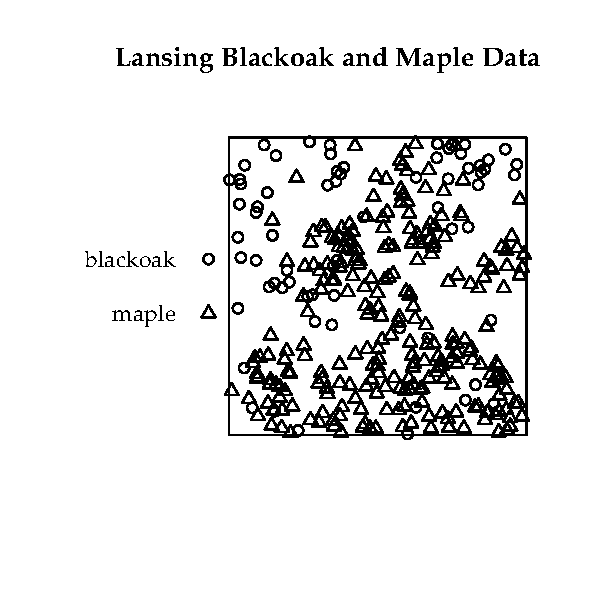
\includegraphics[width=\maxwidth]{figure/prob3-1} 

}



\end{knitrout}

{\it The rectangular region is a unit square. Use the isotropic edge corrected version when applicable below. Answer the following questions. You will be computing several simulation envelopes below. Be patient and keep nsim=99, the default.}

\begin{enumerate}
\item %3a
{\it What does the K function measure?}

The K function measures second order properties (var/cov) of a spatial point process.

According to the help file, the K function estimates the ``inter-dependence" or ``clustering" of a stationary point pattern dataset. The estimate of K is used to infer the spatial pattern.

Paraphrased from the help file:

Where $\lambda$ is the intensity of the process and r is the distance, $\lambda$K(r) is the expected numer of additional random points within a distance of r of a typical random point of X.


\item %3b
{\it It is often easier to interpret the L function than the K function. Based on the L function do the blackoaks appear to be clustered or do they appear to be regularly distributed? Do the maples appear to be clustered or do they appear to be regularly distributed? Justify your answer. Simulation envelopes will help you give a better answer to this question.}

L transforms the K function by taking the square root of K. Under CSR, K is a parabola and by taking the square root of K (L) we can assess deviations from a straight line vs. a parabola when evaluating the CSR assumed hypothesis.

\begin{knitrout}\footnotesize
\definecolor{shadecolor}{rgb}{0.969, 0.969, 0.969}\color{fgcolor}\begin{kframe}
\begin{alltt}
\hlkwd{par}\hlstd{(}\hlkwc{mfrow}\hlstd{=}\hlkwd{c}\hlstd{(}\hlnum{1}\hlstd{,}\hlnum{2}\hlstd{))}
\hlkwd{plot}\hlstd{(}\hlkwd{envelope}\hlstd{(blackoak,}\hlkwc{fun}\hlstd{=}\hlstr{"Lest"}\hlstd{,} \hlkwc{correction}\hlstd{=}\hlstr{"iso"}\hlstd{,} \hlkwc{verbose} \hlstd{=} \hlnum{FALSE}\hlstd{),}
     \hlkwc{main} \hlstd{=} \hlstr{"Blackoak"}\hlstd{)}
\hlkwd{plot}\hlstd{(}\hlkwd{envelope}\hlstd{(maple,} \hlkwc{fun}\hlstd{=}\hlstr{"Lest"}\hlstd{,} \hlkwc{correction}\hlstd{=}\hlstr{"iso"}\hlstd{,} \hlkwc{verbose} \hlstd{=} \hlnum{FALSE}\hlstd{),}
     \hlkwc{main} \hlstd{=} \hlstr{"Maple"}\hlstd{)}
\end{alltt}
\end{kframe}

{\centering 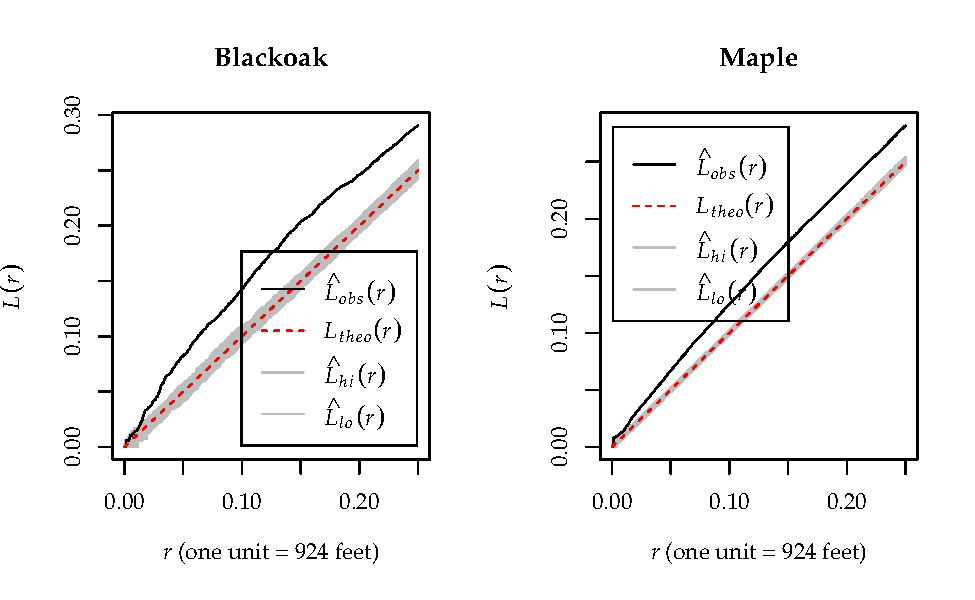
\includegraphics[width=\maxwidth]{figure/prob3b-1} 

}



\end{knitrout}

I used the isotrophic edge corrections. Both the blackoak and maple trees appear to be clustered as the observed number of additional events within almost all distances r is more than expected under CSR for both the blackoak and maple trees. Note that I plotted the simulation envelopes and the observed is outside of the simulation envelopes for most distances as well in both plots.  


\item %3c
{\it Compare the two L functions and discuss whether or not the 2 processes appear to be the same. You can use the results from (a) but you should also look at the difference more formally using the following also provided in an attached script file.}

The two L functions do not appear to be the same as the D function is outside of the simulation envelopes for short distances.

The density plots shows the maple point process and the blackoack point process are near complements of each other, with different patterns and thus we might expect different L functions. Note the frequency of maples is much higher than that of the blackoak within the corresponding clusters.

\begin{knitrout}\footnotesize
\definecolor{shadecolor}{rgb}{0.969, 0.969, 0.969}\color{fgcolor}\begin{kframe}
\begin{alltt}
\hlcom{#r code embedded in midterm}
\hlcom{#chose to output code from file}
\hlcom{# specify radii}
       \hlstd{h}\hlkwb{<-}\hlkwd{seq}\hlstd{(}\hlnum{0}\hlstd{,}\hlnum{.5}\hlstd{,}\hlkwc{l}\hlstd{=}\hlnum{100}\hlstd{)}
       \hlcom{# get coordinates}
       \hlstd{tree.poly}\hlkwb{<-}\hlkwd{list}\hlstd{(}\hlkwc{x}\hlstd{=}\hlkwd{c}\hlstd{(blackoak}\hlopt{$}\hlstd{x,maple}\hlopt{$}\hlstd{x),}\hlkwc{y}\hlstd{=}\hlkwd{c}\hlstd{(blackoak}\hlopt{$}\hlstd{y,maple}\hlopt{$}\hlstd{y))}
       \hlcom{# recompute the K functions}
       \hlstd{kblackoak}\hlkwb{<-}\hlkwd{khat}\hlstd{(}\hlkwd{as.points}\hlstd{(blackoak),}\hlkwd{bboxx}\hlstd{(}\hlkwd{bbox}\hlstd{(}\hlkwd{as.points}\hlstd{(tree.poly))),h)}
       \hlstd{kmaple}\hlkwb{<-}\hlkwd{khat}\hlstd{(}\hlkwd{as.points}\hlstd{(maple),}\hlkwd{bboxx}\hlstd{(}\hlkwd{bbox}\hlstd{(}\hlkwd{as.points}\hlstd{(tree.poly))),h)}
       \hlcom{# get the differences}
       \hlstd{k.diff}\hlkwb{<-}\hlstd{kblackoak} \hlopt{-} \hlstd{kmaple}
       \hlcom{# generate the envelope}
       \hlstd{env}\hlkwb{<-}\hlkwd{Kenv.label}\hlstd{(}\hlkwd{as.points}\hlstd{(blackoak),}\hlkwd{as.points}\hlstd{(maple),}
       \hlkwd{bboxx}\hlstd{(}\hlkwd{bbox}\hlstd{(}\hlkwd{as.points}\hlstd{(tree.poly))),}\hlkwc{nsim}\hlstd{=}\hlnum{99}\hlstd{,}\hlkwc{s}\hlstd{=h,} \hlkwc{quiet} \hlstd{=} \hlnum{TRUE}\hlstd{)}
       \hlcom{# plot the results}
       \hlcom{#plot(h,seq(-0.15,0.05,l=length(h)),type="n",ylab="Kdiff",}
       \hlcom{#main="Envelopes for Kdiff")}
       \hlcom{#lines(h,k.diff)}
       \hlcom{#lines(h,env$low,lty=2)}
       \hlcom{#lines(h,env$up,lty=2)}
       \hlcom{#abline(h=0)}

\hlcom{# r code sent as sepearate file}
\hlstd{Lblackoak}\hlkwb{<-}\hlkwd{envelope}\hlstd{(blackoak,}\hlkwc{fun}\hlstd{=Lest,}\hlkwc{correction}\hlstd{=}\hlstr{"iso"}\hlstd{)}
\end{alltt}
\begin{verbatim}
Generating 99 simulations of CSR  ...
1, 2, 3, 4, 5, 6, 7, 8, 9, 10, 11, 12, 13, 14, 15, 16, 17, 18, 19, 20, 21, 22, 23, 24, 25, 26, 27, 28, 29, 30, 31, 32, 33, 34, 35, 36, 37, 38,
39, 40, 41, 42, 43, 44, 45, 46, 47, 48, 49, 50, 51, 52, 53, 54, 55, 56, 57, 58, 59, 60, 61, 62, 63, 64, 65, 66, 67, 68, 69, 70, 71, 72, 73, 74, 75, 76,
77, 78, 79, 80, 81, 82, 83, 84, 85, 86, 87, 88, 89, 90, 91, 92, 93, 94, 95, 96, 97, 98,  99.

Done.
\end{verbatim}
\begin{alltt}
\hlkwd{plot}\hlstd{(Lblackoak,.}\hlopt{-}\hlstd{r}\hlopt{~}\hlstd{r,}\hlkwc{legend}\hlstd{=F)}
\end{alltt}
\end{kframe}

{\centering 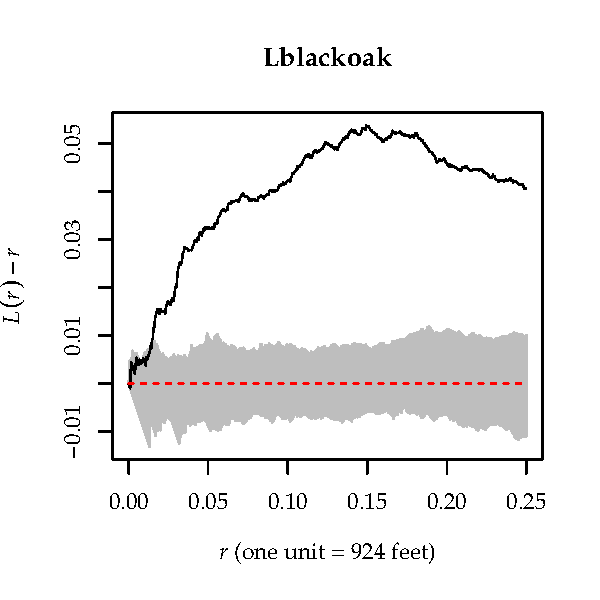
\includegraphics[width=\maxwidth]{figure/prob3c-1} 

}


\begin{kframe}\begin{alltt}
\hlstd{Lmaple}\hlkwb{<-}\hlkwd{envelope}\hlstd{(maple,}\hlkwc{fun}\hlstd{=Lest,}\hlkwc{correctin}\hlstd{=}\hlstr{"iso"}\hlstd{)}
\end{alltt}
\begin{verbatim}
Generating 99 simulations of CSR  ...
1, 2, 3, 4, 5, 6, 7, 8, 9, 10, 11, 12, 13, 14, 15, 16, 17, 18, 19, 20, 21, 22, 23, 24, 25, 26, 27, 28, 29, 30, 31, 32, 33, 34, 35, 36, 37, 38,
39, 40, 41, 42, 43, 44, 45, 46, 47, 48, 49, 50, 51, 52, 53, 54, 55, 56, 57, 58, 59, 60, 61, 62, 63, 64, 65, 66, 67, 68, 69, 70, 71, 72, 73, 74, 75, 76,
77, 78, 79, 80, 81, 82, 83, 84, 85, 86, 87, 88, 89, 90, 91, 92, 93, 94, 95, 96, 97, 98,  99.

Done.
\end{verbatim}
\begin{alltt}
\hlkwd{plot}\hlstd{(Lmaple,.}\hlopt{-}\hlstd{r}\hlopt{~}\hlstd{r,}\hlkwc{legend}\hlstd{=F)}
\end{alltt}
\end{kframe}

{\centering 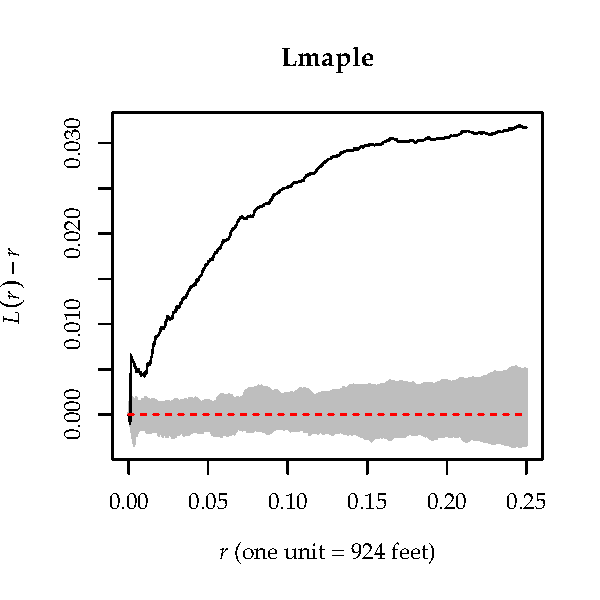
\includegraphics[width=\maxwidth]{figure/prob3c-2} 

}


\begin{kframe}\begin{alltt}
\hlcom{# specify radii}
\hlstd{h}\hlkwb{<-}\hlkwd{seq}\hlstd{(}\hlnum{0}\hlstd{,}\hlnum{.5}\hlstd{,}\hlkwc{l}\hlstd{=}\hlnum{100}\hlstd{)}
\hlcom{# get coordinates}
\hlstd{tree.poly}\hlkwb{<-}\hlkwd{list}\hlstd{(}\hlkwc{x}\hlstd{=}\hlkwd{c}\hlstd{(blackoak}\hlopt{$}\hlstd{x,maple}\hlopt{$}\hlstd{x),}\hlkwc{y}\hlstd{=}\hlkwd{c}\hlstd{(blackoak}\hlopt{$}\hlstd{y,maple}\hlopt{$}\hlstd{y))}
\hlcom{# recompute the K functions}
\hlstd{kblackoak}\hlkwb{<-}\hlkwd{khat}\hlstd{(}\hlkwd{as.points}\hlstd{(blackoak),}\hlkwd{bboxx}\hlstd{(}\hlkwd{bbox}\hlstd{(}\hlkwd{as.points}\hlstd{(tree.poly))),h)}
\hlstd{kmaple}\hlkwb{<-}\hlkwd{khat}\hlstd{(}\hlkwd{as.points}\hlstd{(maple),}\hlkwd{bboxx}\hlstd{(}\hlkwd{bbox}\hlstd{(}\hlkwd{as.points}\hlstd{(tree.poly))),h)}
\hlcom{# get the differences}
\hlstd{k.diff}\hlkwb{<-}\hlstd{kblackoak} \hlopt{-} \hlstd{kmaple}
\hlcom{# generate the envelope}
\hlstd{env}\hlkwb{<-}\hlstd{(}\hlkwd{Kenv.label}\hlstd{(}\hlkwd{as.points}\hlstd{(blackoak),}\hlkwd{as.points}\hlstd{(maple),}
\hlkwd{bboxx}\hlstd{(}\hlkwd{bbox}\hlstd{(}\hlkwd{as.points}\hlstd{(tree.poly))),}\hlkwc{nsim}\hlstd{=}\hlnum{99}\hlstd{,}\hlkwc{s}\hlstd{=h,} \hlkwc{quiet} \hlstd{=} \hlnum{TRUE}\hlstd{))}
\hlcom{# plot the results}
\hlkwd{plot}\hlstd{(h,}\hlkwd{seq}\hlstd{(}\hlopt{-}\hlnum{0.15}\hlstd{,}\hlnum{0.05}\hlstd{,}\hlkwc{l}\hlstd{=}\hlkwd{length}\hlstd{(h)),}\hlkwc{type}\hlstd{=}\hlstr{"n"}\hlstd{,}\hlkwc{ylab}\hlstd{=}\hlstr{"Kdiff"}\hlstd{,}
\hlkwc{main}\hlstd{=}\hlstr{"Envelopes for Kdiff"}\hlstd{)}
\hlkwd{lines}\hlstd{(h,k.diff)}
\hlkwd{lines}\hlstd{(h,env}\hlopt{$}\hlstd{low,}\hlkwc{lty}\hlstd{=}\hlnum{2}\hlstd{)}
\hlkwd{lines}\hlstd{(h,env}\hlopt{$}\hlstd{up,}\hlkwc{lty}\hlstd{=}\hlnum{2}\hlstd{)}
\hlkwd{abline}\hlstd{(}\hlkwc{h}\hlstd{=}\hlnum{0}\hlstd{)}
\end{alltt}
\end{kframe}

{\centering 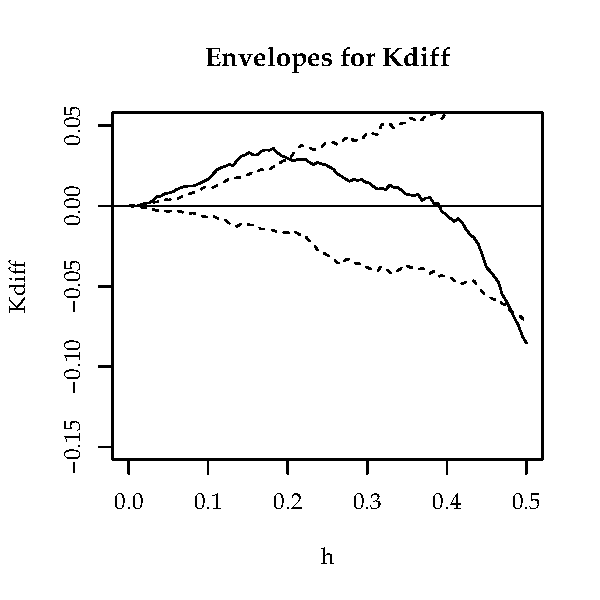
\includegraphics[width=\maxwidth]{figure/prob3c-3} 

}


\begin{kframe}\begin{alltt}
\hlstd{Kenv}\hlkwb{<-}\hlkwd{envelope}\hlstd{(lansing,Kcross,} \hlkwc{i}\hlstd{=}\hlstr{"maple"}\hlstd{,}\hlkwc{j}\hlstd{=}\hlstr{"blackoak"}\hlstd{,} \hlkwc{verbose} \hlstd{=} \hlnum{FALSE}\hlstd{)}
\hlkwd{plot}\hlstd{(Kenv,}\hlkwd{sqrt}\hlstd{(.}\hlopt{/}\hlstd{pi)}\hlopt{-}\hlstd{r}\hlopt{~}\hlstd{r,}\hlkwc{ylab}\hlstd{=}\hlstr{"Lij - h"}\hlstd{,}\hlkwc{main}\hlstd{=}\hlstr{"Cross L Function - Maple
and Black Oak"}\hlstd{,}\hlkwc{legend}\hlstd{=F)}
\end{alltt}
\end{kframe}

{\centering 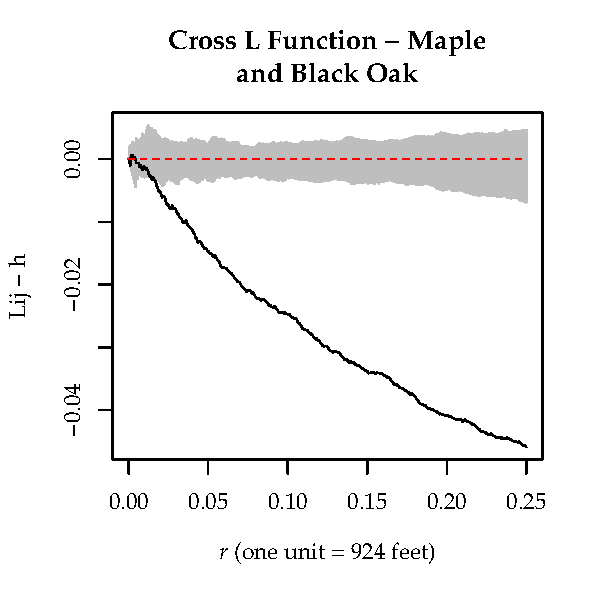
\includegraphics[width=\maxwidth]{figure/prob3c-4} 

}


\begin{kframe}\begin{alltt}
\hlkwd{plot}\hlstd{(}\hlkwd{density}\hlstd{(blackoak))}
\end{alltt}
\end{kframe}

{\centering 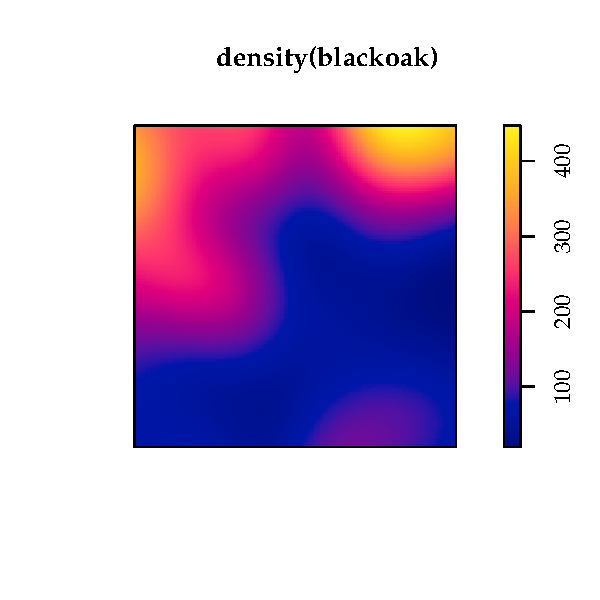
\includegraphics[width=\maxwidth]{figure/prob3c-5} 

}


\begin{kframe}\begin{alltt}
\hlkwd{plot}\hlstd{(}\hlkwd{density}\hlstd{(maple))}
\end{alltt}
\end{kframe}

{\centering 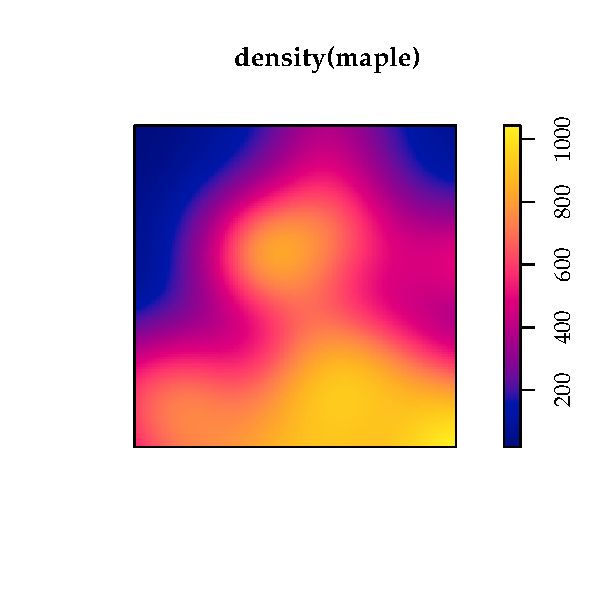
\includegraphics[width=\maxwidth]{figure/prob3c-6} 

}



\end{knitrout}

\item %3d
{\it Plot Lij − h versus h for black oaks and maples.}
\begin{knitrout}\footnotesize
\definecolor{shadecolor}{rgb}{0.969, 0.969, 0.969}\color{fgcolor}\begin{kframe}
\begin{alltt}
\hlstd{Kplot}\hlkwb{<-}\hlkwd{envelope}\hlstd{(lansing,Kcross,}\hlkwc{i}\hlstd{=}\hlstr{"blackoak"}\hlstd{,}\hlkwc{j}\hlstd{=}\hlstr{"maple"}\hlstd{,} \hlkwc{verbose} \hlstd{=} \hlnum{FALSE}\hlstd{)}
\hlkwd{plot}\hlstd{(Kplot,}\hlkwd{sqrt}\hlstd{(.}\hlopt{/}\hlstd{pi)}\hlopt{-}\hlstd{r}\hlopt{~}\hlstd{r,}\hlkwc{ylab}\hlstd{=}\hlstr{"Lij - h"}\hlstd{,}\hlkwc{main}\hlstd{=}\hlstr{"Cross L Function"}\hlstd{,}\hlkwc{legend}\hlstd{=F)}
\end{alltt}
\end{kframe}

{\centering 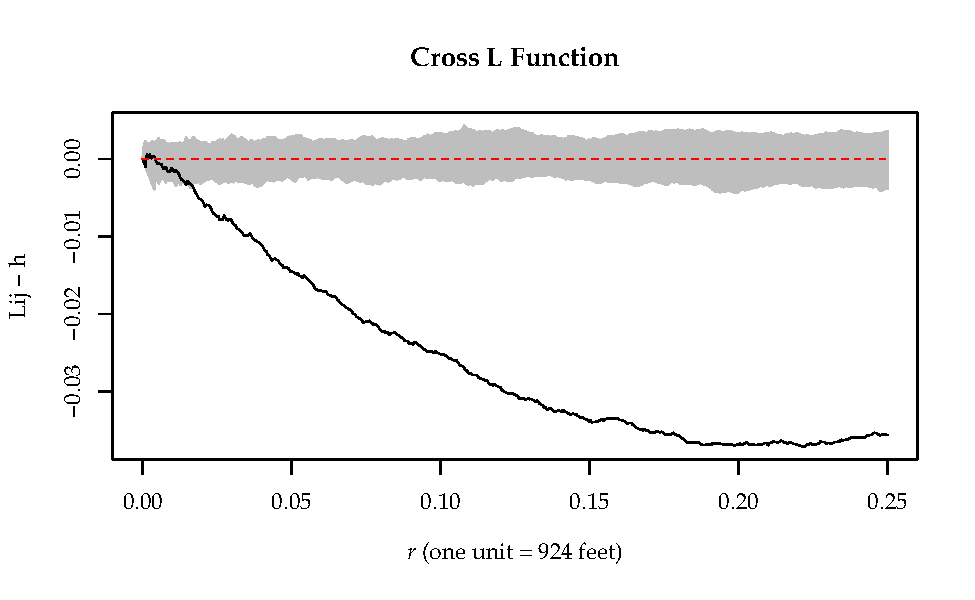
\includegraphics[width=\maxwidth]{figure/prob3d-1} 

}



\end{knitrout}

{\it What type of relationship between the point patterns of the two species of trees is indicated by this plot? Justify your answer.}

Because the observed Lij - h curve is below the theoretical (including below the corresponding simulation envelopes), the plot indicates the two species of trees are inhibiting the growth of each other, e.g., we do not expect to see many blackoaks near a cluster of maples.

\item %3e
{\it Based on the above, comment on the null hypotheses of independence and random labeling.}

{\bf Independence}
$H_{o}$: The spatial locations and the binary marks are determed simultaneously and independently of one another, meaning as $K_{ij}(h)$ is defined in the notes at the top of page 38 can be simplified to $K(h)$ = $\pi*h^{2}$. This implies the expected number of additional trees within distance h of one species of trees is the same regardless of which species is of interest and only depends on the distance considered, h.

The plot in (d) suggests evidence against the null hypothesis of independence and evidence for inhibition.

Mathematically this is violated because under the null hypothesis $E[K_{ij}(h)]$ = h.

{\bf Random Labelling}
$H_{o}$: Locations arise from a univariate point process and the labels are determined by a process similar to random thinning, where the label is determined by a Bernoulli trial at each location. Where 1 indicates a blackoak and 2 indicates a maple, the null hypothesis corresponds to $K_{11} = K_{22} = K_{12} = K$.

The Kdiff plot in (c) suggests $K_{11} \neq K_{22}$, which should hold under random labelling. Therefore, random labelling of the process is also not suggested.

%Plots of $L_{11}$ and $L_{22}$ both indicate spatial clustering. Inhibition of the growth of one species might suggest clustered growth of another species, also suggesting clustering by species. These three do not suggest $K_{11}$, $K_{22}$, $K_{12}$, nor K differ and so we would not find evidence against random labelling. 

\end{enumerate}

\item %4
{\it You were sent the wheat data set on a previous homework assignment. You want to predict the value of Z (yield) at an arbitrary location. Assume a pure nugget effect model.}

\begin{enumerate}
\item %4a
{\it What are the kriging weights and what is the predicted value?}

\begin{knitrout}\footnotesize
\definecolor{shadecolor}{rgb}{0.969, 0.969, 0.969}\color{fgcolor}\begin{kframe}
\begin{alltt}
\hlkwd{plot}\hlstd{(wheat.variog} \hlkwb{<-} \hlkwd{variog}\hlstd{(wheat.geodat),}
     \hlkwc{main} \hlstd{=} \hlstr{"Empirical Semivariogram"}\hlstd{)}
\end{alltt}
\begin{verbatim}
variog: computing omnidirectional variogram
\end{verbatim}
\end{kframe}

{\centering 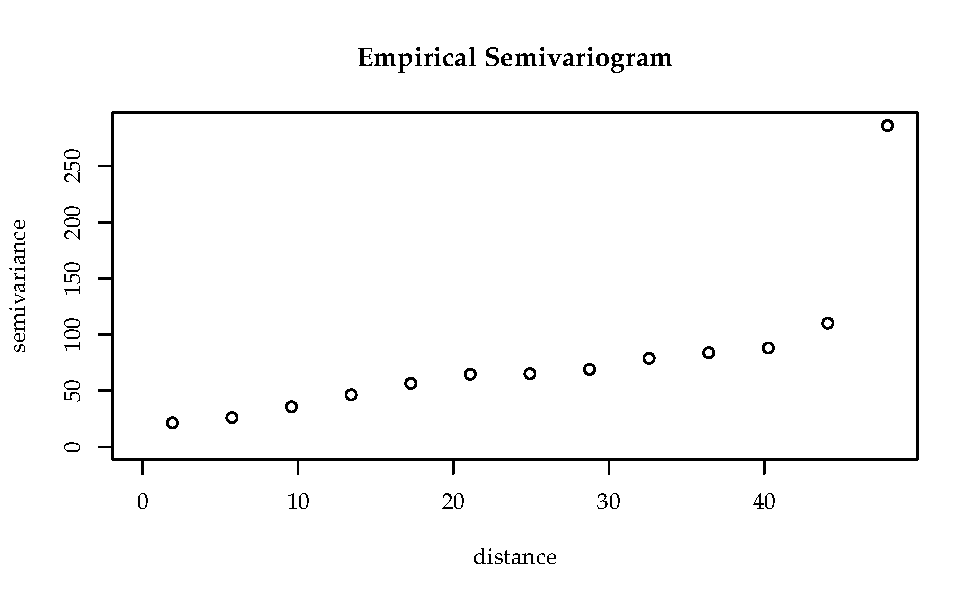
\includegraphics[width=\maxwidth]{figure/prob4a-1} 

}


\begin{kframe}\begin{alltt}
\hlstd{wheat.dist} \hlkwb{<-} \hlkwd{as.matrix}\hlstd{(}\hlkwd{dist}\hlstd{(wheat.geodat}\hlopt{$}\hlstd{coords))}
\hlstd{d} \hlkwb{<-} \hlkwd{dim}\hlstd{(wheat.dist)}

\hlcom{# what is the nugget?}
\hlcom{# using empirical right now}
\hlstd{Sigma} \hlkwb{<-} \hlkwd{diag}\hlstd{(}\hlkwd{var}\hlstd{(wheat.geodat}\hlopt{$}\hlstd{data),} \hlkwc{nrow} \hlstd{= d[}\hlnum{1}\hlstd{],} \hlkwc{ncol} \hlstd{= d[}\hlnum{1}\hlstd{])}

\hlstd{a} \hlkwb{<-} \hlkwd{c}\hlstd{(}\hlkwd{rep}\hlstd{(}\hlnum{1}\hlstd{,d[}\hlnum{1}\hlstd{]))}

\hlstd{Sigma.star} \hlkwb{<-} \hlkwd{as.matrix}\hlstd{(}\hlkwd{cbind}\hlstd{((}\hlkwd{rbind}\hlstd{(Sigma,a)),}\hlkwd{c}\hlstd{(a,}\hlnum{0}\hlstd{)),}
                        \hlkwc{nrow} \hlstd{=} \hlnum{225}\hlstd{,} \hlkwc{ncol} \hlstd{=} \hlnum{225}\hlstd{)}
\hlkwd{str}\hlstd{(Sigma.star)}
\end{alltt}
\begin{verbatim}
 num [1:225, 1:225] 55.5 0 0 0 0 ...
 - attr(*, "dimnames")=List of 2
  ..$ : chr [1:225] "" "" "" "" ...
  ..$ : NULL
\end{verbatim}
\begin{alltt}
\hlkwd{dim}\hlstd{(Sigma.star)}
\end{alltt}
\begin{verbatim}
[1] 225 225
\end{verbatim}
\begin{alltt}
\hlstd{newx} \hlkwb{<-} \hlkwd{runif}\hlstd{(}\hlnum{1}\hlstd{,}\hlkwd{min}\hlstd{(wheat.geodat}\hlopt{$}\hlstd{coords[,}\hlnum{1}\hlstd{]),} \hlkwd{max}\hlstd{(wheat.geodat}\hlopt{$}\hlstd{coords[,}\hlnum{1}\hlstd{]))}
\hlstd{newy} \hlkwb{<-} \hlkwd{runif}\hlstd{(}\hlnum{1}\hlstd{,}\hlkwd{min}\hlstd{(wheat.geodat}\hlopt{$}\hlstd{coords[,}\hlnum{2}\hlstd{]),} \hlkwd{max}\hlstd{(wheat.geodat}\hlopt{$}\hlstd{coords[,}\hlnum{2}\hlstd{]))}

\hlstd{sigma.vec} \hlkwb{<-} \hlkwd{as.matrix}\hlstd{(}\hlkwd{dist}\hlstd{(}\hlkwd{rbind}\hlstd{(wheat.geodat}\hlopt{$}\hlstd{coords,} \hlkwd{c}\hlstd{(newx,newy))))}
\hlstd{sigma.vec} \hlkwb{<-} \hlstd{sigma.vec[}\hlnum{225}\hlstd{,]}

\hlstd{sigma.star} \hlkwb{<-} \hlkwd{c}\hlstd{(}\hlkwd{rep}\hlstd{(}\hlnum{0}\hlstd{,}\hlnum{224}\hlstd{),}\hlnum{1}\hlstd{)}
\hlstd{lambda.star} \hlkwb{<-} \hlkwd{solve}\hlstd{(Sigma.star)} \hlopt \hlstd{sigma.star}
\hlstd{lambda.star} \hlkwb{<-} \hlkwd{round}\hlstd{(lambda.star,}\hlnum{4}\hlstd{)}

\hlstd{p.ok} \hlkwb{<-} \hlkwd{sum}\hlstd{(lambda.star[}\hlopt{-}\hlnum{225}\hlstd{]}\hlopt{*}\hlstd{wheat.geodat}\hlopt{$}\hlstd{data)}
\hlcom{# the predicted value is just the mean}

\hlcom{# note in pure nugget cov.pars shouldn't matter}
\end{alltt}
\end{kframe}
\end{knitrout}

The predicted value is the mean, 25.731225, and all 224 of the weights are 0.0045.

\item %4b
{\it What is the estimate of the sill?}

Note the sill is the nugget in a pure nugget model. The estimate of the sill is the estimate of the nugget, which was 55.5051753.

\item %4c
{\it What is the kriging standard error (note that this is a {\bf prediction} error)?}

\begin{knitrout}\footnotesize
\definecolor{shadecolor}{rgb}{0.969, 0.969, 0.969}\color{fgcolor}\begin{kframe}
\begin{alltt}
\hlstd{c0} \hlkwb{<-} \hlstd{Sigma[}\hlnum{1}\hlstd{,}\hlnum{1}\hlstd{]}

\hlstd{sigma2.ok} \hlkwb{<-} \hlstd{c0} \hlopt{-} \hlkwd{sum}\hlstd{(lambda.star}\hlopt{*}\hlstd{sigma.star)}
\hlcom{# took sqrt of sigma2.ok for se}
\end{alltt}
\end{kframe}
\end{knitrout}

The kriging standard error is 7.4667915.
\end{enumerate}

\item %5

{\it Carbon-Nitrogen data example: We looked at estimating the semivariogram of the residuals from a simple linear regression model of total carbon on total nitrogen in class. We used gls to do this (as part of incorporating a spatial covariance structure into the regression) specifying an {\bf exponential} covariance model and estimating the parameters using both {\bf maximum likelihood and REML}. Let's check to see what the lik.fit function in the geoR package would return as parameter estimates (nugget, practical range, and partial sill) and see if the results are comparable. Some of the relevant R code is included in the attached script file. Compare the estimates on page 11 of the Spatial Regression notes and the estimates you get out of lik.fit. Use the same starting values.}

\begin{knitrout}\footnotesize
\definecolor{shadecolor}{rgb}{0.969, 0.969, 0.969}\color{fgcolor}\begin{kframe}
\begin{alltt}
\hlstd{CN.dat} \hlkwb{<-} \hlkwd{read.table}\hlstd{(}\hlstr{"CN.dat"}\hlstd{,} \hlkwc{header} \hlstd{=} \hlnum{TRUE}\hlstd{)}

\hlstd{pred.grid}\hlkwb{<-}\hlkwd{expand.grid}\hlstd{(}\hlkwd{seq}\hlstd{(}\hlopt{-}\hlnum{50}\hlstd{,}\hlnum{550}\hlstd{,}\hlkwc{l}\hlstd{=}\hlnum{100}\hlstd{),}\hlkwd{seq}\hlstd{(}\hlopt{-}\hlnum{15}\hlstd{,}\hlnum{330}\hlstd{,}\hlkwc{l}\hlstd{=}\hlnum{100}\hlstd{))}

\hlstd{TC.geodat}\hlkwb{<-}\hlkwd{as.geodata}\hlstd{(CN.dat,}\hlkwc{coords.col}\hlstd{=}\hlnum{1}\hlopt{:}\hlnum{2}\hlstd{,}\hlkwc{data.col}\hlstd{=}\hlnum{4}\hlstd{)}


\hlcom{# Problem 5}

\hlcom{# get the CN data}
\hlkwd{names}\hlstd{(CN.dat)}\hlkwb{<-}\hlkwd{c}\hlstd{(}\hlstr{"x"}\hlstd{,}\hlstr{"y"}\hlstd{,}\hlstr{"tn"}\hlstd{,}\hlstr{"tc"}\hlstd{,}\hlstr{"cn"}\hlstd{)}
\hlcom{#attach(CN.dat)}
\hlstd{CN.lm}\hlkwb{<-}\hlkwd{lm}\hlstd{(tc}\hlopt{~}\hlstd{tn,} \hlkwc{data} \hlstd{= CN.dat)}
\hlstd{resids}\hlkwb{<-}\hlkwd{residuals}\hlstd{(CN.lm)}
\hlcom{# convert to a geodata object }
\hlstd{resids.dat}\hlkwb{<-}\hlkwd{cbind}\hlstd{(CN.dat}\hlopt{$}\hlstd{x,CN.dat}\hlopt{$}\hlstd{y,resids)}
\hlstd{resids.dat}\hlkwb{<-}\hlkwd{data.frame}\hlstd{(resids.dat)}
\hlkwd{names}\hlstd{(resids.dat)}\hlkwb{<-}\hlkwd{c}\hlstd{(}\hlstr{"x"}\hlstd{,}\hlstr{"y"}\hlstd{,}\hlstr{"resids"}\hlstd{)}
\hlstd{resids.geodat}\hlkwb{<-}\hlkwd{as.geodata}\hlstd{(resids.dat,}\hlkwc{coords.col}\hlstd{=}\hlnum{1}\hlopt{:}\hlnum{2}\hlstd{,}\hlkwc{data.col}\hlstd{=}\hlnum{3}\hlstd{)}


\hlcom{# now fit the models. }

\hlcom{# gls initial params = c(range,nugget/sill)}

\hlcom{# likfit initial params = c(sill-nugget, range/3)}

\hlcom{# problem: NEED sill and nugget, not proportion}
\hlcom{# look back at variog on p.9 to get corresponding}
\hlcom{# starting values}
\hlcom{# looks like sill is about 1.2}
\hlcom{# this means nugget is about 1.2*0.4=0.48}
\hlcom{# needed to do this to have similar starting values}
\hlcom{# as those in the notes}

\hlstd{range.init} \hlkwb{<-} \hlnum{15}
\hlstd{nugget.init} \hlkwb{<-} \hlnum{0.48}
\hlstd{sill.init} \hlkwb{<-} \hlnum{1.2}

\hlstd{resids.ML} \hlkwb{<-} \hlkwd{likfit}\hlstd{(resids.geodat, resids.geodat}\hlopt{$}\hlstd{coords,}
                     \hlstd{resids.geodat}\hlopt{$}\hlstd{data,} \hlkwc{cov.model} \hlstd{=} \hlstr{"exponential"}\hlstd{,}
                     \hlkwc{ini.cov.pars} \hlstd{=} \hlkwd{c}\hlstd{(sill.init}\hlopt{-}\hlstd{nugget.init,range.init}\hlopt{/}\hlnum{3}\hlstd{),}
                    \hlkwc{fix.nugget} \hlstd{=} \hlnum{FALSE}\hlstd{,} \hlkwc{nugget} \hlstd{= nugget.init,}
                    \hlkwc{lik.method} \hlstd{=} \hlstr{"ML"}\hlstd{,} \hlkwc{hessian} \hlstd{=} \hlnum{TRUE}\hlstd{,} \hlkwc{messages} \hlstd{=} \hlnum{FALSE}\hlstd{)}

\hlstd{resids.REML} \hlkwb{<-} \hlkwd{likfit}\hlstd{(resids.geodat, resids.geodat}\hlopt{$}\hlstd{coords,}
                     \hlstd{resids.geodat}\hlopt{$}\hlstd{data,} \hlkwc{cov.model} \hlstd{=} \hlstr{"exponential"}\hlstd{,}
                     \hlkwc{ini.cov.pars} \hlstd{=} \hlkwd{c}\hlstd{(sill.init}\hlopt{-}\hlstd{nugget.init,range.init}\hlopt{/}\hlnum{3}\hlstd{),}
                    \hlkwc{fix.nugget} \hlstd{=} \hlnum{FALSE}\hlstd{,} \hlkwc{nugget} \hlstd{= nugget.init,}
                    \hlkwc{lik.method} \hlstd{=} \hlstr{"REML"}\hlstd{,} \hlkwc{hessian} \hlstd{=} \hlnum{TRUE}\hlstd{,} \hlkwc{messages} \hlstd{=} \hlnum{FALSE}\hlstd{)}

\hlstd{resids.ML}\hlopt{$}\hlstd{cov.pars}
\end{alltt}
\begin{verbatim}
[1]  0.001065496 47.224029867
\end{verbatim}
\begin{alltt}
\hlstd{resids.ML}\hlopt{$}\hlstd{nugget}
\end{alltt}
\begin{verbatim}
[1] 0.0005981685
\end{verbatim}
\begin{alltt}
\hlstd{resids.REML}\hlopt{$}\hlstd{cov.pars}
\end{alltt}
\begin{verbatim}
[1]  0.001133522 56.242656929
\end{verbatim}
\end{kframe}
\end{knitrout}



{\bf REML}

The table on p.11 of the notes using gls includes the proportion of the sill that is due to the nugget effect (estimated to be 0.356 with a confidence interval of 0.194 to 0.559). The gls function estimated the nugget effect to be 0.000621. Likfit estimated the nugget effect to be \ensuremath{6.2\times 10^{-4}}, and so the results are similar.

Gls estimated the sill to be 0.00177 with a confidence interval ranging from 0.0013 to 0.00215. Likfit estimated the partial sill to be 0.00113 and thus the sill to be 0.00113 +  \ensuremath{6.2\times 10^{-4}} = 0.00175. Again, the likfit estimate falls within the confidence interval based on the gls estimate and the results between gls and likfit are comparable.

Gls estimated the practical range to be 175.089 with a confidence interval ranging from 58.49 to 524.131. Likfit estimated the practical range to be 3*56.24 = 168.73. We see again the results are comparable. 

%I was able to figure out how to calculate the standard error of phi from likfit, which was phiREMLse. A confidence interval using this the se of phi from likfit would be similar in width to the confidence interval using the se of phi from gls.


{\bf MAXIMUM LIKLIHOOD}

Gls estimated the nugget to be $0.00167*0.363$ = \ensuremath{6.06\times 10^{-4}} (proportion of the sill that is due to the nugget was estimated to be 0.363 with a confidence interval of 0.196 to 0.571). Likfit estimated the nugget to be \ensuremath{5.98\times 10^{-4}}.

Gls estimated the sill to be 0.00167 with a confidence interval ranging from 0.00121 to 0.0029. Likfit estimated the partial sill to be 0.00107 and thus the sill to be 0.00107 +  \ensuremath{6\times 10^{-4}} = 0.00166. 

Gls estimated the practical range to be 144.929 with a confidence interval ranging from 58.588 to 358.515. Likfit estimated the practical range to be 3*47.22 = 141.67. 

%My attempt of a confidence interval forphi from likfit was ciML[1] to ciML[2]. A confidence interval using this the se of phi from likfit is would be similar in width to the confidence interval using the se of phi from gls.

We see again the results are comparable for all three parameters whether using likfit and ML or gls and ML.


\end{enumerate}
\end{document}

